\documentclass{beamer}
\usetheme{Boadilla}
\usepackage{graphicx}
\usepackage[final]{animate}
\usepackage{breqn}
\usepackage{xcolor}
\usepackage{booktabs}
\usepackage{pgf}
\usepackage{caption}

% change format of enumerated lists
\setbeamertemplate{enumerate items}[default]
\setbeamertemplate{navigation symbols}{}

% macros
\newcommand{\emtxt}[1]{\textbf{\textit{{\color{mypal4} #1}}}}

% change font size for figure captions
\setbeamerfont{caption}{size=\scriptsize}

\usefonttheme{serif}

% custom colors
\definecolor{mypal1}{HTML}{FFF7FD}\definecolor{mypal2}{HTML}{D7CEE9}\definecolor{mypal3}{HTML}{76A6D0}\definecolor{mypal4}{HTML}{00828B}\definecolor{mypal5}{HTML}{004533}
% setup

% get online bib file

\setbeamercolor{title}{fg=mypal5} % main title
\setbeamercolor{frametitle}{fg=mypal4, bg=mypal2} % frame titles
\setbeamercolor{structure}{fg=mypal4} % bottom banner
\setbeamercolor{normal text}{fg=mypal5}
\usebackgroundtemplate{
\includegraphics[height=\paperheight,width=\paperwidth]{fig/back_tmp.pdf}}

\usepackage{Sweave}
\begin{document}
\Sconcordance{concordance:Beck_etal_CERF_2019.tex:Beck_etal_CERF_2019.Rnw:%
1 22 1 1 20 1 1 1 13 1 1 1 6 7 1 1 0 242 1}


\title[Tracking SF Bay Water Quality]{Tracking San Francisco Bay water quality using generalized additive models in an R Shiny framework}
\author[Beck et al.]{Marcus W. Beck\inst{1} \and Ian Wren\inst{2} \and Rebecca Murphy\inst{3} \and \\ Perry de Valpine\inst{4} \and David Senn\inst{5}}

\institute[TBEP]{$^1$Tampa Bay Estuary Program\\ $^2$San Francisco Baykeeper \\$^3$University of Maryland at Cheseapeake Bay Program \\$^4$University of California Berkeley \\$^5$San Francisco Estuary Institute}

\date{Nov. 4, 2019}

\titlegraphic{
\vspace{-0.1in}
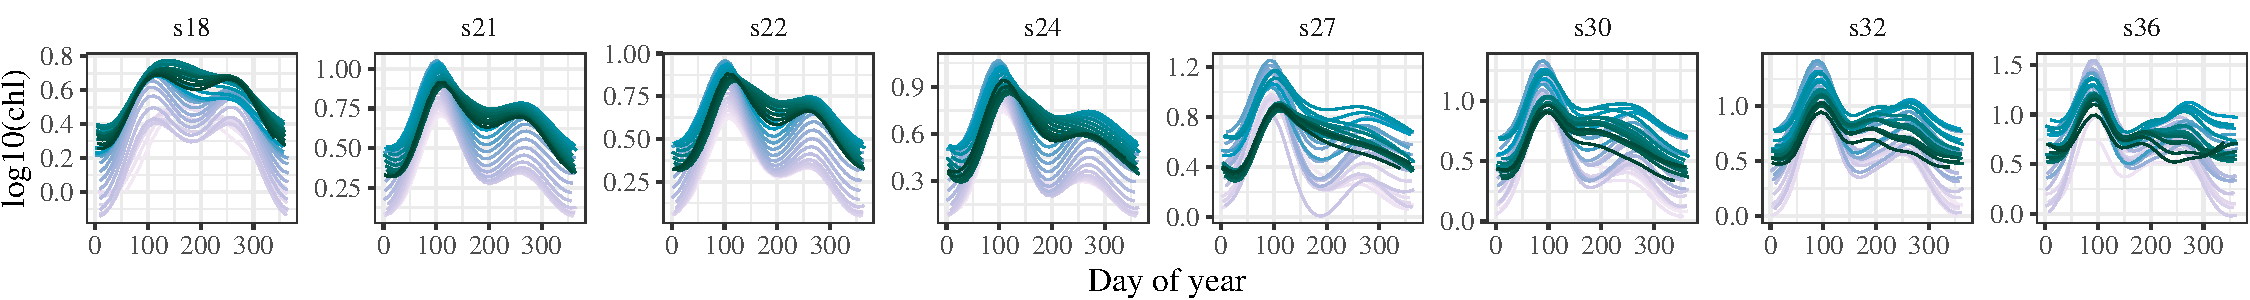
\includegraphics[width=\linewidth]{fig/titlegraph.pdf}
}

%%%%%%
\begin{frame}
% \vspace{0.2in}
\titlepage
\end{frame}

\section{Background}

%%%%%%
\begin{frame}{\textbf{Why do we care about trends?} \hspace{0pt plus 1 filll} $\vcenter{\hbox{
\includegraphics[width=0.15\paperwidth]{fig/logo.png}}}$}
\begin{itemize}
\onslide<1->
\item Provide information on natural variation of water quality parameters \\~\\
\begin{itemize}
\item What are the 1\textsuperscript{st} order principles that describe a system? \\~\\
\end{itemize}
\onslide<2->
\item Document historical changes in response to management actions \\~\\
\begin{itemize}
\item Did investments make a difference? \\~\\
\end{itemize}
\onslide<3->
\item Anticipate future changes with proposed restoration or management \\~\\
\begin{itemize}
\item Can we understand the past to predict the future?
\end{itemize}
\end{itemize}
\end{frame}

%%%%%%
\begin{frame}{\textbf{Trends vary in space and time} \hspace{0pt plus 1 filll} $\vcenter{\hbox{
\includegraphics[width=0.15\paperwidth]{fig/logo.png}}}$}
\centerline{\emtxt{Observed data represent effects of many processes}}
\vspace{0.15in}
\centerline{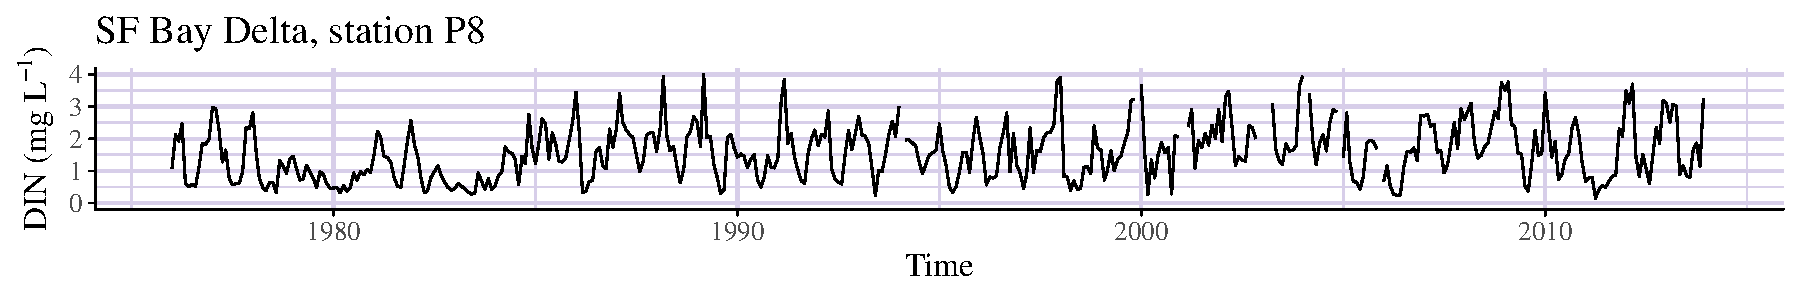
\includegraphics[width = \textwidth]{fig/ts_ex.pdf}}
\vspace{0.15in}
\begin{columns}[t]
\begin{column}{0.3\textwidth}
{\bf \underline{\emtxt{Climate}}}\\
precipitation\\
temperature\\
wind events\\
ENSO effects
\end{column}
\begin{column}{0.3\textwidth}
{\bf \underline{\emtxt{Local}}}\\
light/turbidity\\
residence time\\
invasive species\\
trophic effects
\end{column}
\begin{column}{0.3\textwidth}
{\bf \underline{\emtxt{Regional/historical}}}\\
watershed inputs\\
point sources\\
management actions
flow changes
\end{column}
\end{columns}
\end{frame}

%%%%%%
\begin{frame}{\textbf{Must translate data into information} \hspace{0pt plus 1 filll} $\vcenter{\hbox{
\includegraphics[width=0.15\paperwidth]{fig/logo.png}}}$}
\onslide<+->
\centerline{\emtxt{Observed data represents effects of many processes}}
\vspace{0.15in}
\centerline{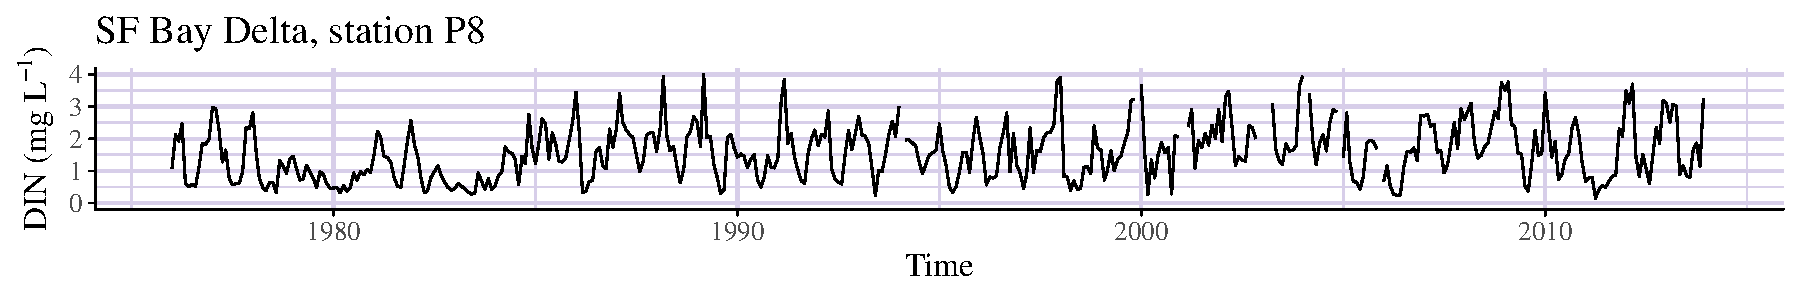
\includegraphics[width = \textwidth]{fig/ts_ex.pdf}}
\centerline{\emtxt{Models should describe components to evaluate effects}}
\vspace{-0.1in}
\begin{columns}[t]
\begin{column}{0.5\textwidth}
\onslide<+->{
\centerline{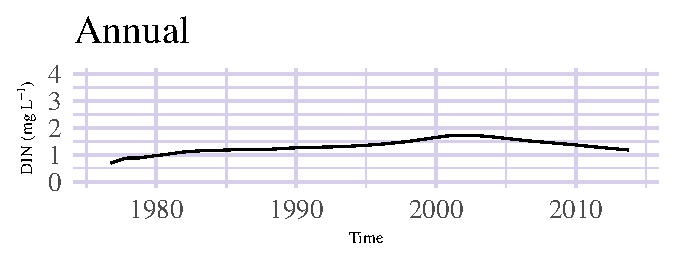
\includegraphics[width = 0.8\textwidth]{fig/schematic2.pdf}}
\centerline{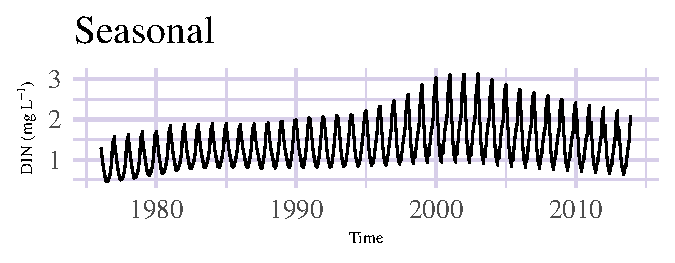
\includegraphics[width = 0.8\textwidth]{fig/schematic3.pdf}}
}
\end{column}
\begin{column}{0.5\textwidth}
\onslide<+->{
\centerline{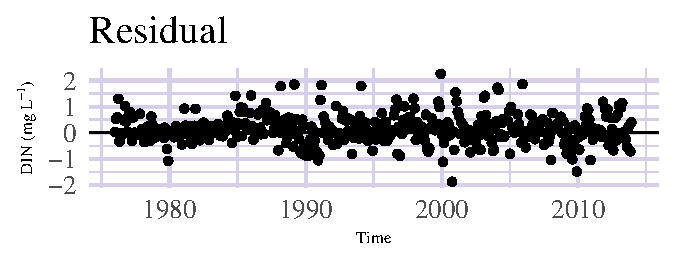
\includegraphics[width = 0.8\textwidth]{fig/schematic4.pdf}}
\centerline{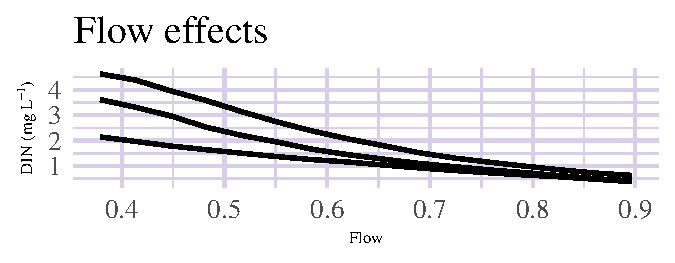
\includegraphics[width = 0.8\textwidth]{fig/schematic5.pdf}}
}
\end{column}
\end{columns}
\end{frame}

\section{Methods}

%%%%%%
\begin{frame}[t]{\textbf{South San Francisco Bay} \hspace{0pt plus 1 filll} $\vcenter{\hbox{
\includegraphics[width=0.15\paperwidth]{fig/logo.png}}}$}
\begin{columns}
\begin{column}{0.5\textwidth}
\begin{itemize}
\onslide<1->
\item A high-nutrient, high-turbidity, low-productivity system {\tiny \cite{Cole84,Alpine88}} \\~\\
\onslide<2->
\item Recent increases observed in summer/fall chl-a {\tiny \cite{Cloern07,Cloern12b}} \\~\\
\onslide<3->
\item Nutrient Management Strategy (NMS) to characterize status/trends and management needs 
\end{itemize}
\end{column}
\begin{column}{0.5\textwidth}
\onslide<1->
\centerline{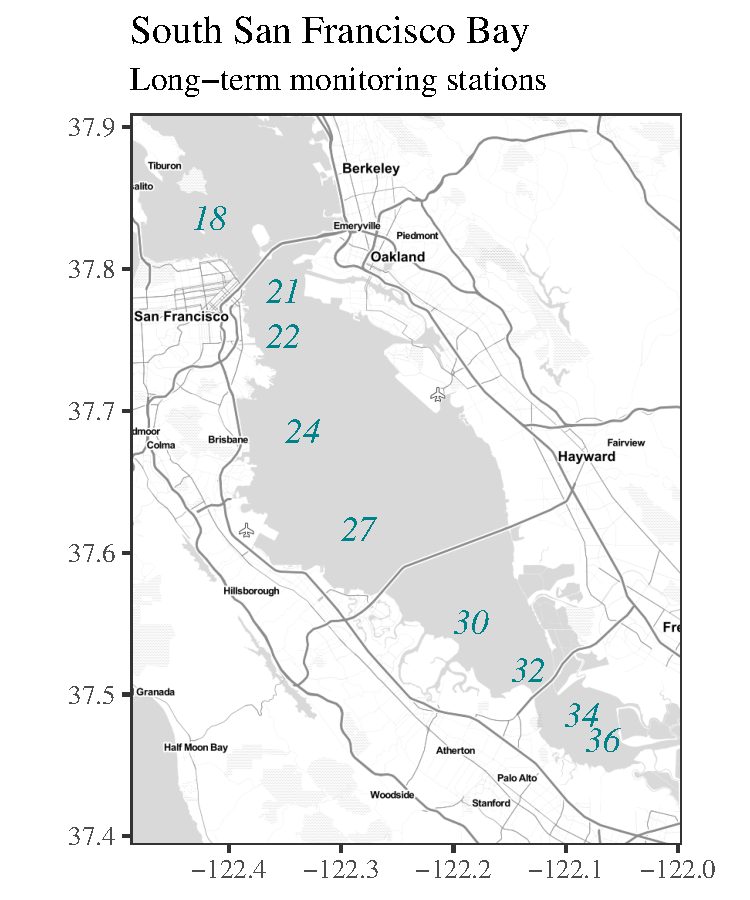
\includegraphics[width = \textwidth]{fig/map.pdf}}
\end{column}
\end{columns}
\end{frame}

%%%%%%
\begin{frame}[t]{\textbf{South San Francisco Bay} \hspace{0pt plus 1 filll} $\vcenter{\hbox{
\includegraphics[width=0.15\paperwidth]{fig/logo.png}}}$}
\begin{columns}
\begin{column}{0.5\textwidth}
\onslide<1->
Questions of concern: \\~\\
\begin{itemize}
\onslide<2->
\item Since changes are visually apparent, which are significant?  \\~\\
\onslide<3->
\item What has been the estimated rate and direction of any linear or non-monotonic change? \\~\\
\onslide<4->
\item Do any of these changes coincide with changes in other water quality parameters?
\end{itemize}
\end{column}
\begin{column}{0.5\textwidth}
\onslide<1->
\centerline{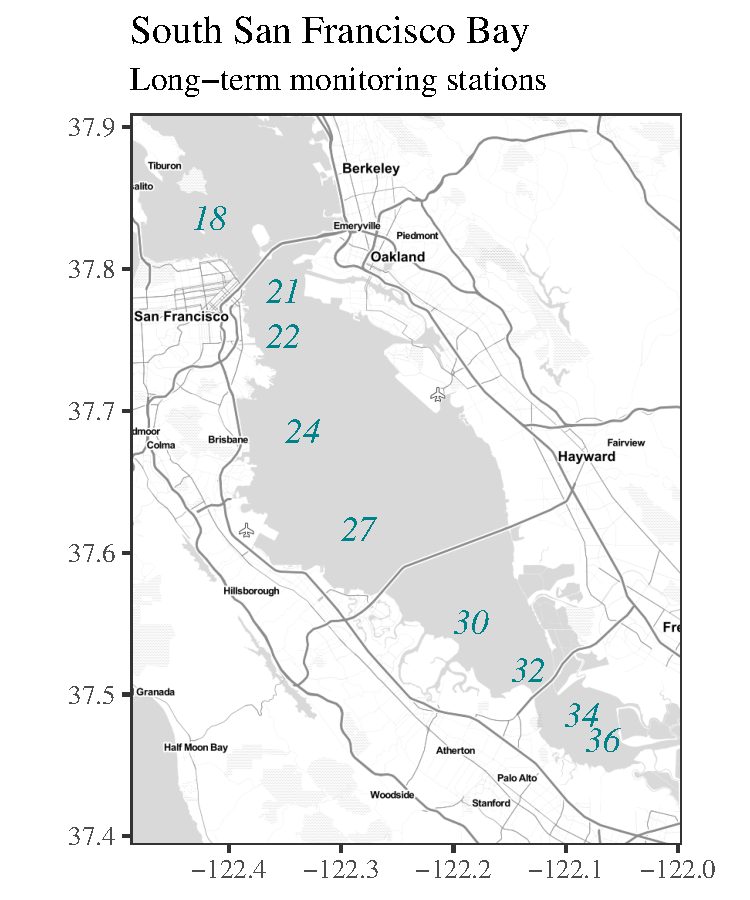
\includegraphics[width = \textwidth]{fig/map.pdf}}
\end{column}
\end{columns}
\end{frame}

%%%%%%
\begin{frame}{\textbf{Application of additive models} \hspace{0pt plus 1 filll} $\vcenter{\hbox{
\includegraphics[width=0.15\paperwidth]{fig/logo.png}}}$}
\begin{itemize}
\onslide<1->
\item The Chesapeake Bay Program (CBP) has been wrestling with similar issues {\tiny \cite{Beck17,Murphy19}} \\~\\
\onslide<2->
\item We applied Generalized Additive Models (GAMs) as implemented by CBP to characterize long-term trends at nine stations over thirty years in South SF Bay \\~\\
\onslide<3->
\item For each station, chlorophyll was modelled as a function of annual and seasonal changes over time using four model structures {\tiny \cite[baytrends R package]{Murphy19b}}\\~\\
\begin{itemize}
\onslide<4->
\item \texttt{gam0}: chl $\sim$ year + s(doy)
\onslide<5->
\item \texttt{gam1}: chl $\sim$ year + s(doy) + s(year)
\onslide<6->
\item \texttt{gam2}: chl $\sim$ year + s(doy) + s(year) + ti(doy, year)
\onslide<7->
\item \texttt{gam6}: chl $\sim$ year + s(doy) + s(year, k = large)
\end{itemize}
\end{itemize}
\end{frame}

%%%%%%
\begin{frame}{\textbf{Application of additive models} \hspace{0pt plus 1 filll} $\vcenter{\hbox{
\includegraphics[width=0.15\paperwidth]{fig/logo.png}}}$}
% \begin{columns}
% \begin{column}{0.7\textwidth}
% \begin{overprint}
\only<1>{\texttt{gam0}: chl $\sim$ year + s(doy)}
\only<2>{\texttt{gam1}: chl $\sim$ year + s(doy) + s(year)}
\only<3>{\texttt{gam2}: chl $\sim$ year + s(doy) + s(year) + ti(doy, year)}
\only<4>{\texttt{gam6}: chl $\sim$ year + s(doy) + s(year, k = large)}
% \end{overprint}
% \end{column}
% \begin{column}{0.3\textwidth}
\onslide<1->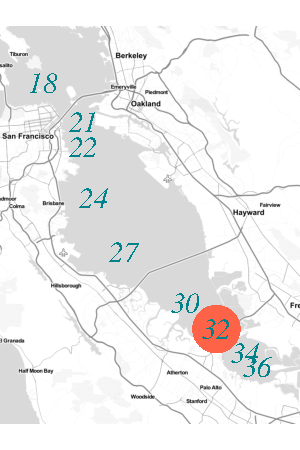
\includegraphics[width =0.1\textwidth]{fig/mapins32.pdf}
\vfill
% \end{column}
% \end{columns}
\begin{columns}
\begin{column}{0.5\textwidth}
\begin{figure}
\begin{overprint}
\onslide<1>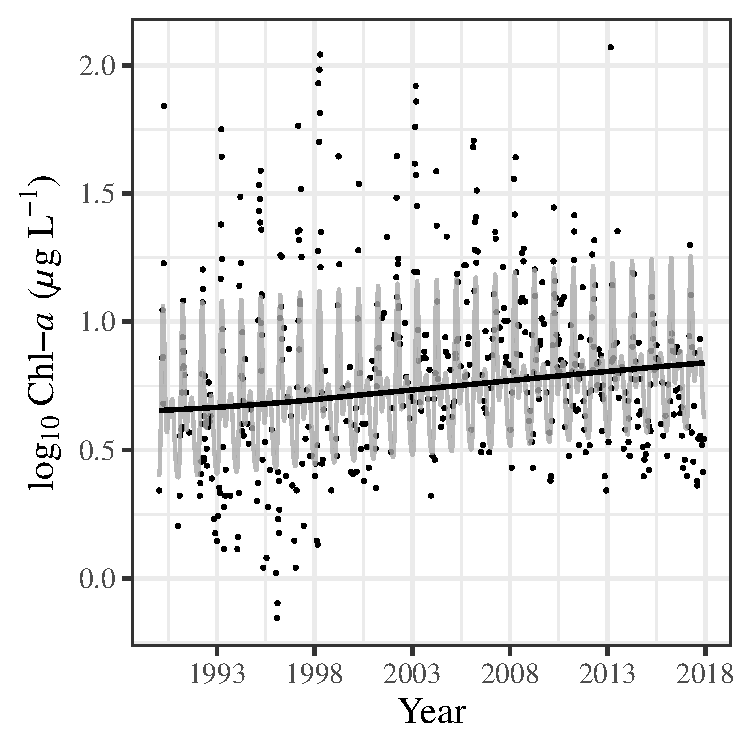
\includegraphics[width = \textwidth, page = 1]{fig/gamex.pdf}
\onslide<2>\includegraphics[width = \textwidth, page = 2]{fig/gamex.pdf}
\onslide<3>\includegraphics[width = \textwidth, page = 3]{fig/gamex.pdf}
\onslide<4>\includegraphics[width = \textwidth, page = 4]{fig/gamex.pdf}
\end{overprint}
\end{figure}
\end{column}
\begin{column}{0.5\textwidth}
\begin{figure}
\begin{overprint}
\onslide<1>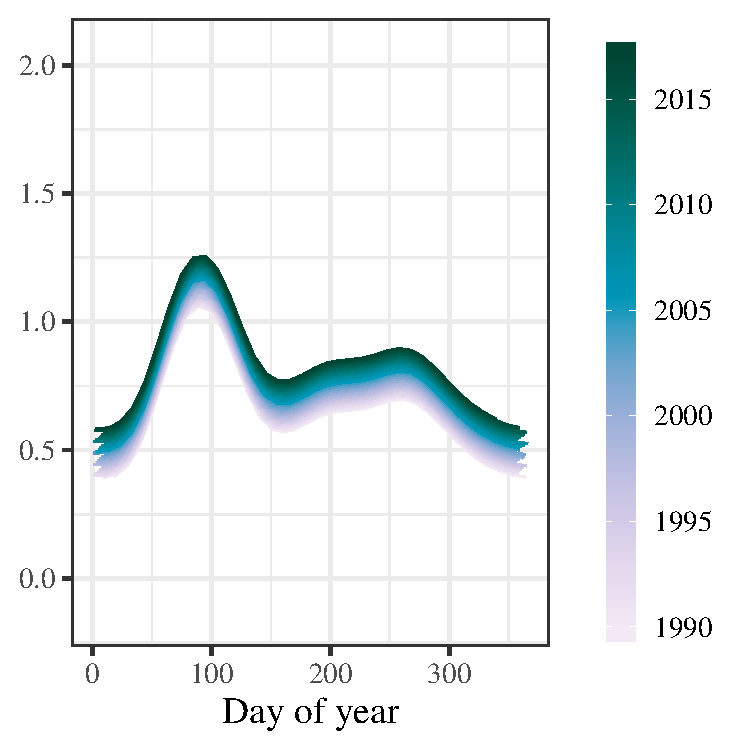
\includegraphics[width = \textwidth, page = 1]{fig/gamex2.pdf}
\onslide<2>\includegraphics[width = \textwidth, page = 2]{fig/gamex2.pdf}
\onslide<3>\includegraphics[width = \textwidth, page = 3]{fig/gamex2.pdf}
\onslide<4>\includegraphics[width = \textwidth, page = 4]{fig/gamex2.pdf}
\end{overprint}
\end{figure}
\end{column}
\end{columns}
\end{frame}

\section{Results}

%%%%%%
\begin{frame}{\textbf{Application of additive models} \hspace{0pt plus 1 filll} $\vcenter{\hbox{
\includegraphics[width=0.15\paperwidth]{fig/logo.png}}}$}
\vspace{-0.2in}
\begin{center}
\animategraphics[controls,width=\linewidth]{12}{fig/anidoy}{}{} %frame rate is 12 per/sec
\end{center}
\end{frame}

%%%%%%
\begin{frame}{\textbf{Application of additive models} \hspace{0pt plus 1 filll} $\vcenter{\hbox{
\includegraphics[width=0.15\paperwidth]{fig/logo.png}}}$}
\vspace{-0.15in}
\begin{center}
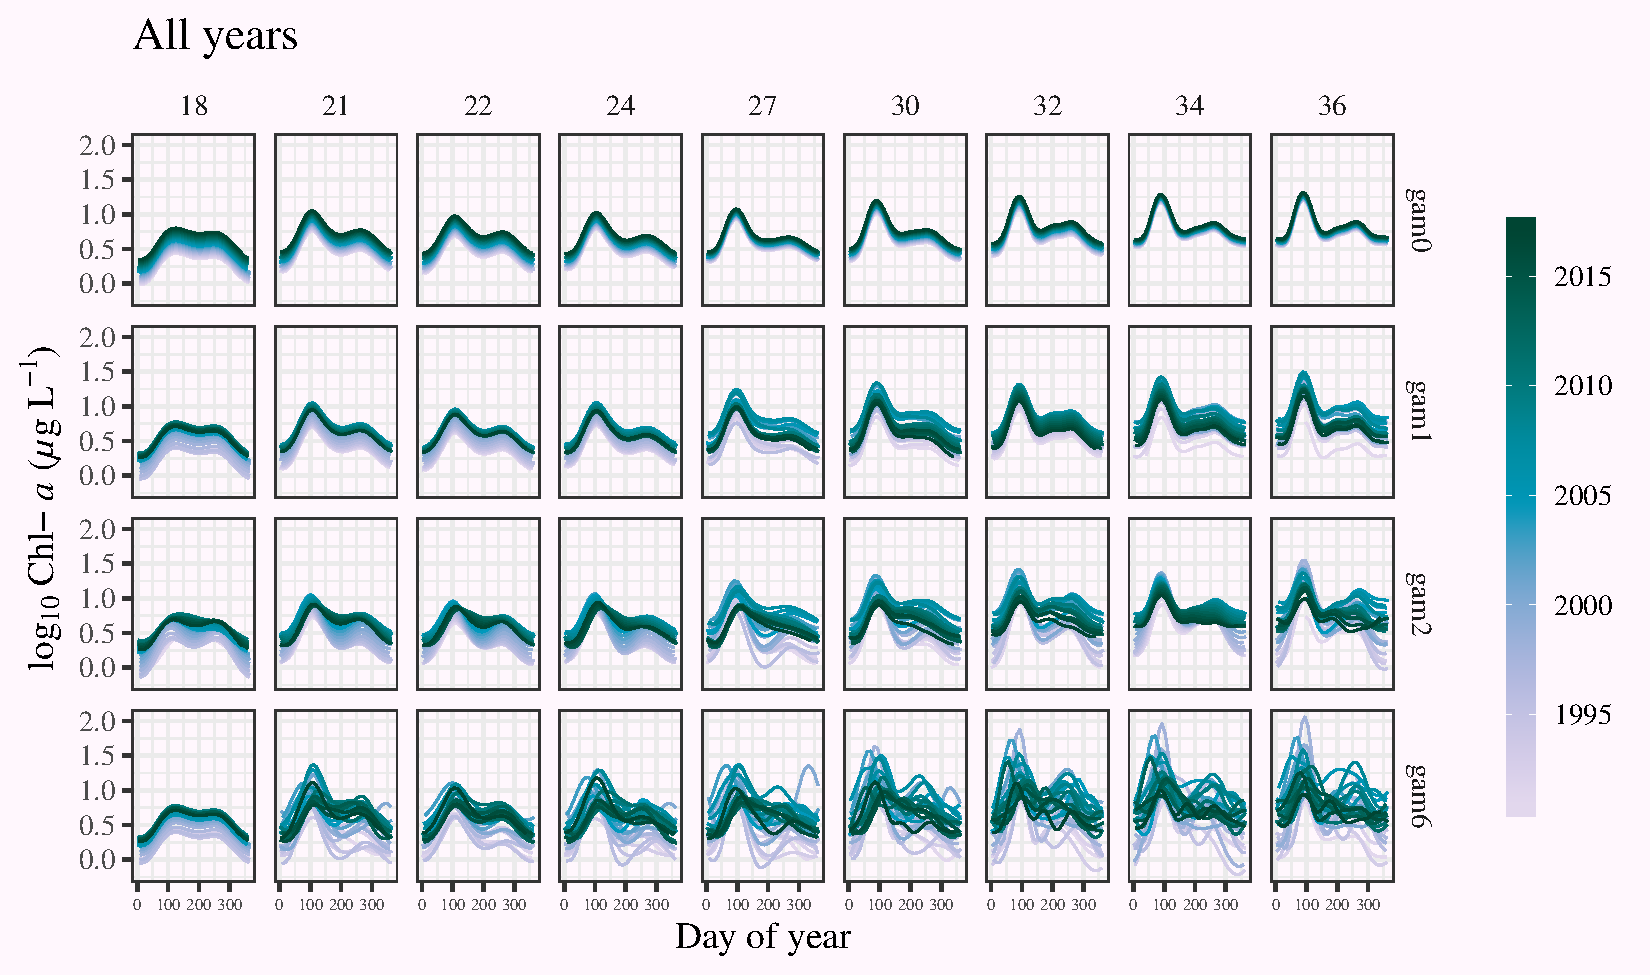
\includegraphics[width=\textwidth]{fig/alldoy.pdf}
\end{center}
\end{frame}

%%%%%%
\begin{frame}{\textbf{Application of additive models} \hspace{0pt plus 1 filll} $\vcenter{\hbox{
\includegraphics[width=0.15\paperwidth]{fig/logo.png}}}$}

\onslide<1->
%latex.default(totab, file = "", rowlabel = "Model", size = "tiny",     rowname = NULL, cgroup = c("", "Stations (north to south)"),     n.cgroup = c(1, 9), caption = "Generalized cross-validation (GCV) summary statistics by station and model")%
\begin{table}[!tbp]
{\tiny
\caption{Generalized cross-validation (GCV) summary statistics by station and model\label{totab}} 
\begin{center}
\begin{tabular}{lclllllllll}
\hline\hline
\multicolumn{1}{c}{\bfseries }&\multicolumn{1}{c}{\bfseries }&\multicolumn{9}{c}{\bfseries Stations (north to south)}\tabularnewline
\cline{3-11}
\multicolumn{1}{c}{Model}&\multicolumn{1}{c}{}&\multicolumn{1}{c}{18}&\multicolumn{1}{c}{21}&\multicolumn{1}{c}{22}&\multicolumn{1}{c}{24}&\multicolumn{1}{c}{27}&\multicolumn{1}{c}{30}&\multicolumn{1}{c}{32}&\multicolumn{1}{c}{34}&\multicolumn{1}{c}{36}\tabularnewline
\hline
gam0&&-117.5&-30.6&-20.6&38.9&174.4&205.5&232.9&256.6&238.7\tabularnewline
gam1&&-138.8&-89.3&-70.3&-18.7&104.1&111.5&162.6&196&182\tabularnewline
gam2&&\textbf{\color{mypal3} -141.8}&-147.3&\textbf{\color{mypal3} -116.4}&-98.5&4&49.6&108.1&189.9&147.2\tabularnewline
gam6&&-139.5&\textbf{\color{mypal3} -235.2}&-116.3&\textbf{\color{mypal3} -176.8}&\textbf{\color{mypal3} -92.1}&\textbf{\color{mypal3} -115.9}&\textbf{\color{mypal3} -149}&\textbf{\color{mypal3} -3.3}&\textbf{\color{mypal3} -65.5}\tabularnewline
\hline
\end{tabular}\end{center}}
\end{table}
\onslide<2->
%latex.default(totab, file = "", rowlabel = "Model", size = "tiny",     rowname = NULL, cgroup = c("", "Stations (north to south)"),     n.cgroup = c(1, 9), caption = "R-squared summary statistics by station and model")%
\begin{table}[!tbp]
{\tiny
\caption{R-squared summary statistics by station and model\label{totab}} 
\begin{center}
\begin{tabular}{lclllllllll}
\hline\hline
\multicolumn{1}{c}{\bfseries }&\multicolumn{1}{c}{\bfseries }&\multicolumn{9}{c}{\bfseries Stations (north to south)}\tabularnewline
\cline{3-11}
\multicolumn{1}{c}{Model}&\multicolumn{1}{c}{}&\multicolumn{1}{c}{18}&\multicolumn{1}{c}{21}&\multicolumn{1}{c}{22}&\multicolumn{1}{c}{24}&\multicolumn{1}{c}{27}&\multicolumn{1}{c}{30}&\multicolumn{1}{c}{32}&\multicolumn{1}{c}{34}&\multicolumn{1}{c}{36}\tabularnewline
\hline
gam0&&0.47&0.41&0.37&0.37&0.33&0.36&0.32&0.31&0.32\tabularnewline
gam1&&0.51&0.48&0.43&0.44&0.43&0.48&0.41&0.41&0.43\tabularnewline
gam2&&\textbf{\color{mypal3} 0.53}&0.54&0.48&0.53&0.54&0.54&0.49&0.41&0.48\tabularnewline
gam6&&0.51&\textbf{\color{mypal3} 0.68}&\textbf{\color{mypal3} 0.54}&\textbf{\color{mypal3} 0.66}&\textbf{\color{mypal3} 0.68}&\textbf{\color{mypal3} 0.72}&\textbf{\color{mypal3} 0.75}&\textbf{\color{mypal3} 0.69}&\textbf{\color{mypal3} 0.75}\tabularnewline
\hline
\end{tabular}\end{center}}
\end{table}\end{frame}

%%%%%%
\begin{frame}{\textbf{Conclusions from additive models} \hspace{0pt plus 1 filll} $\vcenter{\hbox{
\includegraphics[width=0.15\paperwidth]{fig/logo.png}}}$}
\begin{itemize}
\onslide<1->
\item More complex models provided more ``parsimonious'' fit \\~\\
\begin{itemize}
\item Non-monotonic trends were obvious 
\item Interactions between year/season were common \\~\\
\end{itemize}
\onslide<2->
\item Clear demarcation of annual and seasonal trends allowed a description of the separate components \\~\\
\begin{itemize}
\item Annual trends showed increase, with some decreases in recent period of record
\item Change in dominance between spring/fall peaks were observed \\~\\
\end{itemize}
\end{itemize}
\onslide<3->
\centerline{\emtxt{How can this information support decision-making??}}
\end{frame}

%%%%%%
\begin{frame}{\textbf{Shiny interactive web platform} \hspace{0pt plus 1 filll} $\vcenter{\hbox{
\includegraphics[width=0.15\paperwidth]{fig/logo.png}}}$}
\vspace{-0.15in}
\begin{center}
\emtxt{https://sccwrp.shinyapps.io/sfbaytrends}
\end{center}
\centerline{\fbox{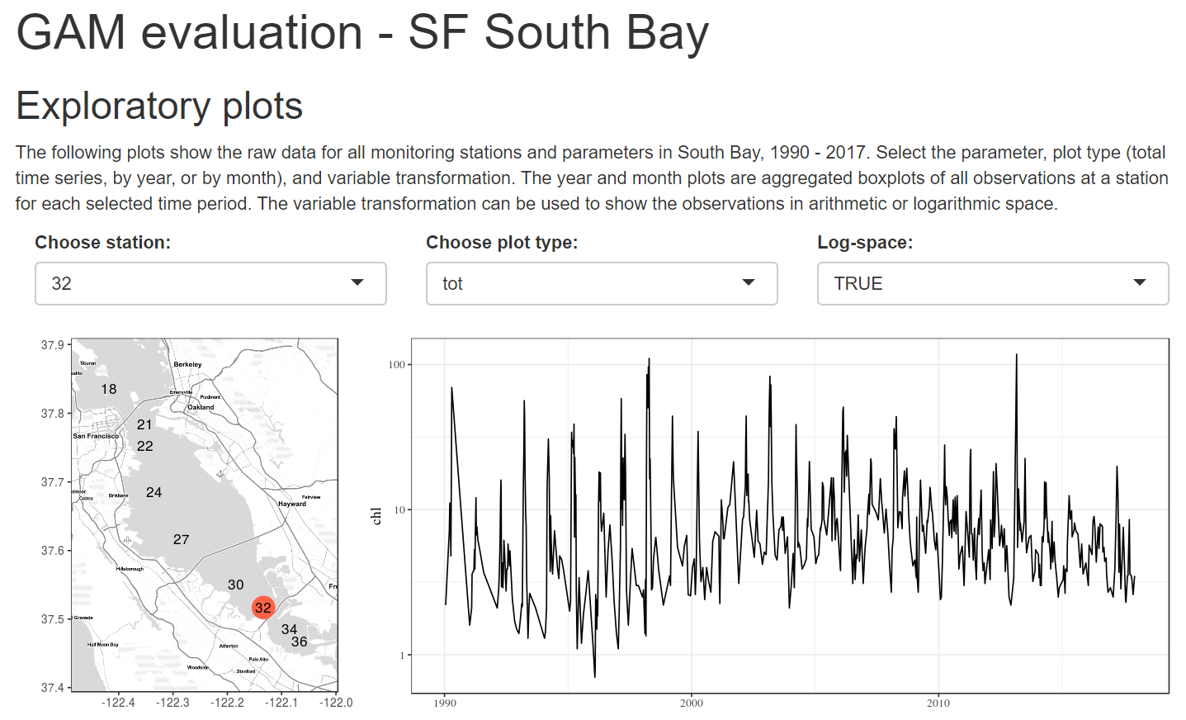
\includegraphics[width = 0.85\textwidth]{fig/shiny1.png}}}
\end{frame}

%%%%%%
\begin{frame}{\textbf{Shiny interactive web platform} \hspace{0pt plus 1 filll} $\vcenter{\hbox{
\includegraphics[width=0.15\paperwidth]{fig/logo.png}}}$}
\vspace{-0.15in}
\begin{center}
\emtxt{Explore results for each station, by model}
\end{center}
\centerline{\fbox{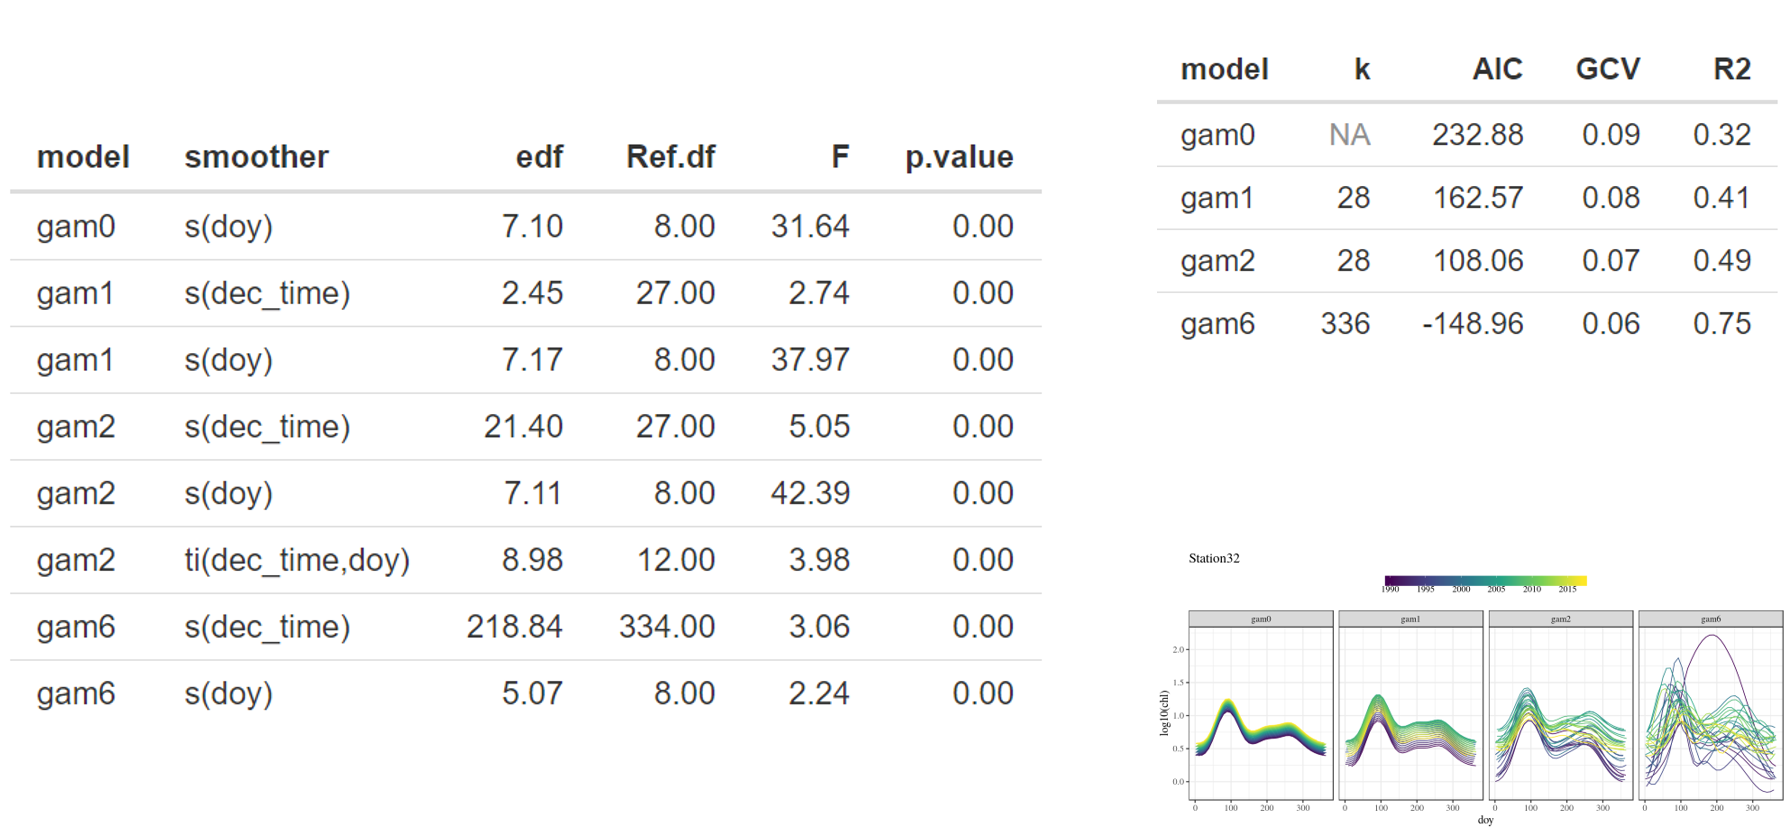
\includegraphics[width = 0.85\textwidth]{fig/shiny2.png}}}
\end{frame}

%%%%%%
\begin{frame}{\textbf{Shiny interactive web platform} \hspace{0pt plus 1 filll} $\vcenter{\hbox{
\includegraphics[width=0.15\paperwidth]{fig/logo.png}}}$}
\vspace{-0.25in}
\begin{center}
\emtxt{Perform trend tests with selected years}
\end{center}
\begin{overprint}
\onslide<1>\centerline{\fbox{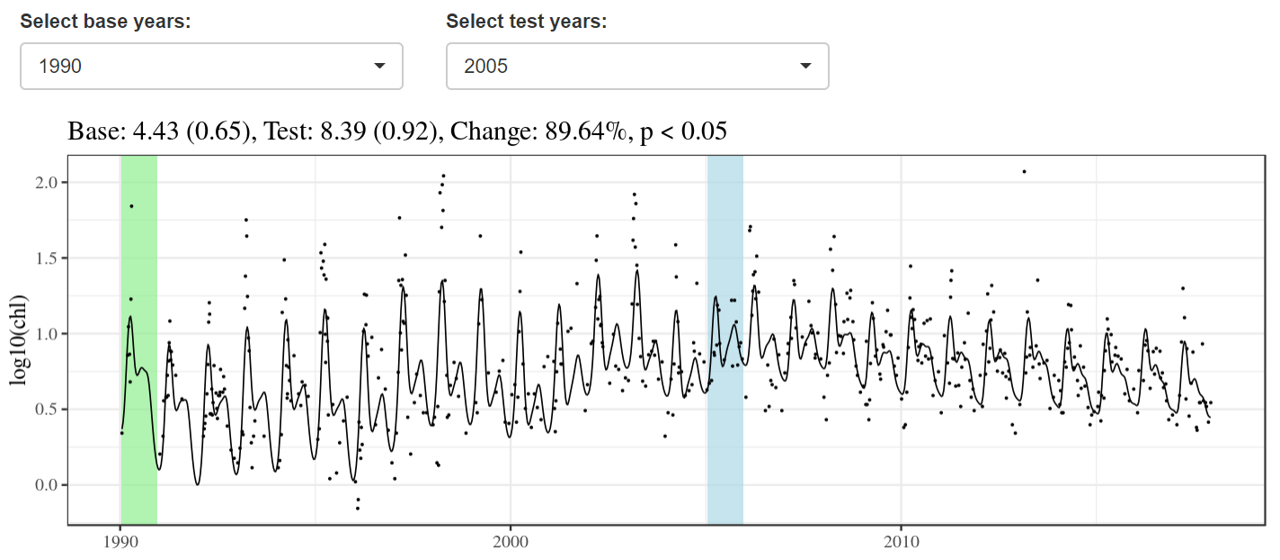
\includegraphics[width = 0.95\textwidth]{fig/shiny3a.png}}}
\onslide<2>\centerline{\fbox{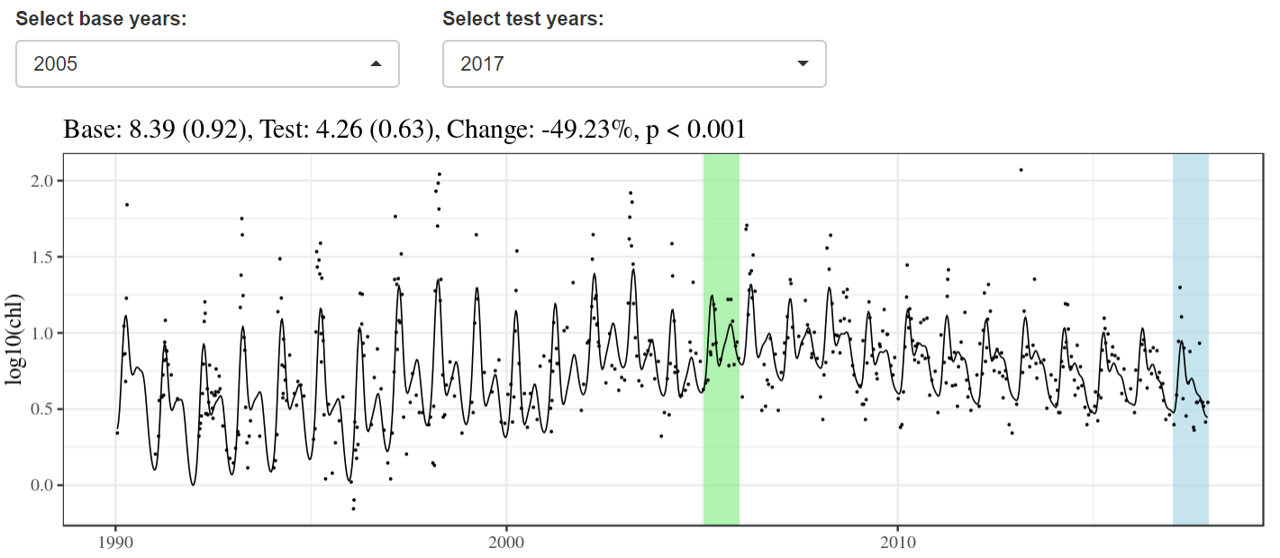
\includegraphics[width = 0.95\textwidth]{fig/shiny3b.png}}}
\end{overprint}
\end{frame}

%%%%%%
\begin{frame}{\textbf{Shiny interactive web platform} \hspace{0pt plus 1 filll} $\vcenter{\hbox{
\includegraphics[width=0.15\paperwidth]{fig/logo.png}}}$}
\vspace{-0.15in}
\begin{center}
\emtxt{Evaluate trends between years, by season}
\end{center}
\begin{overprint}
\onslide<1>\centerline{\fbox{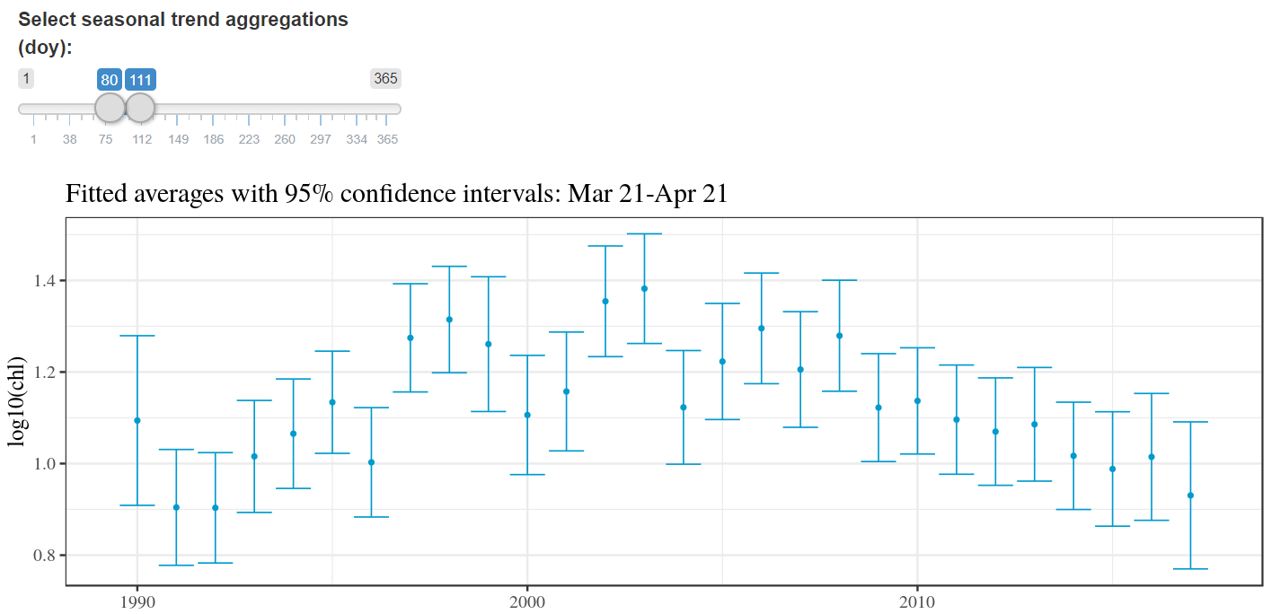
\includegraphics[width = 0.95\textwidth]{fig/shiny4a.png}}}
\onslide<2>\centerline{\fbox{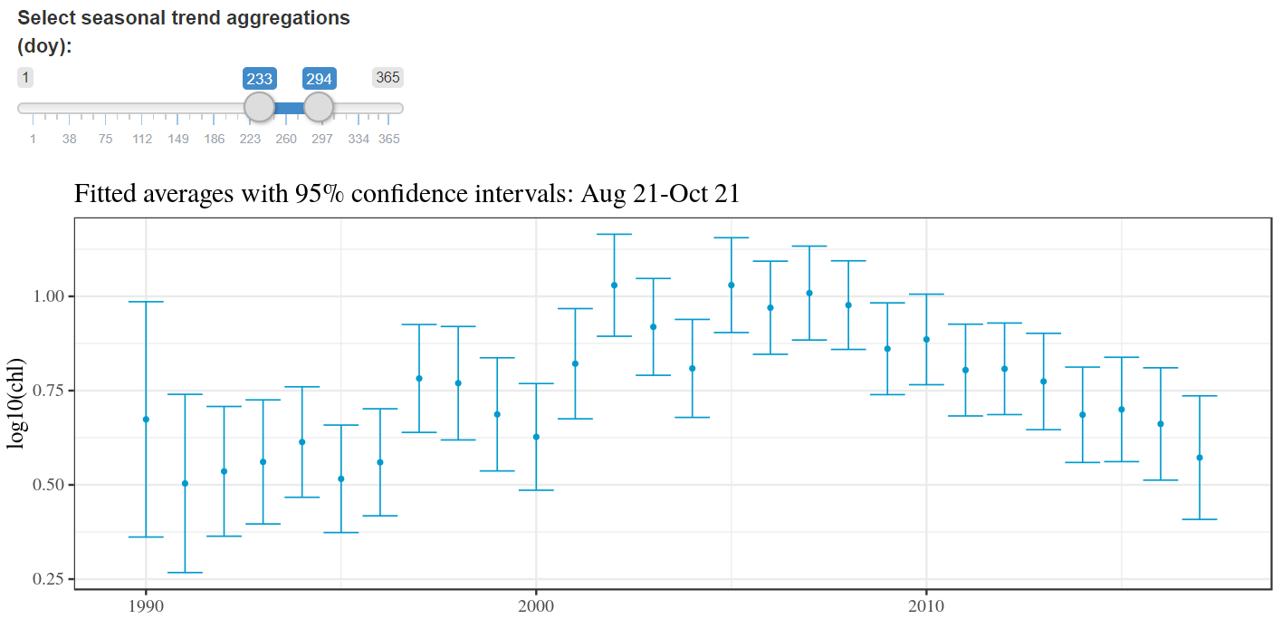
\includegraphics[width = 0.95\textwidth]{fig/shiny4b.png}}}
\end{overprint}
\end{frame}

\section{Conclusions}

%%%%%%
\begin{frame}{\textbf{Summary and next steps} \hspace{0pt plus 1 filll} $\vcenter{\hbox{
\includegraphics[width=0.15\paperwidth]{fig/logo.png}}}$}
\begin{itemize}
\onslide<1->
\item This analysis was a proof of concept \\~\\
\begin{itemize}
\item Does the GAM approach developed by the CBP transfer to SF Bay?
\item Do additional considerations need to be made? \\~\\
\end{itemize}
\onslide<2->
\item Shiny platform helps communicate results to stakeholder  \\~\\
\begin{itemize}
\item Which station, model, and time period do I care about?
\item How can I understand limitations of the different models? \\~\\
\end{itemize}
\onslide<3->
\item Follow-up work: \\~\\
\begin{itemize}
\item Extend to other locations in the Bay
\item Explore trend analysis of aggregated stations
\item Incorporate additional variables - as response or as explanatory
\end{itemize}
\end{itemize}
\end{frame}

%%%%%%
\begin{frame}
Acknowledgments and contact info:\\~\\
\begin{columns}
\begin{column}{0.9\textwidth}
{\footnotesize
Research staff and employees at the San Francisco Estuary Institute, Delta Regional Monitoring Program, Southern California Coastal Water Research Project, and the Tampa Bay Estuary Program
}
\end{column}
\end{columns}
\vfill
\begin{columns}
\begin{column}{0.6\textwidth}
\begin{center}
\hfill

\includegraphics[width=0.3\linewidth]{fig/sfei1.png}
\hfill

\includegraphics[width=0.3\linewidth]{fig/sfei2.png} \\~\\
\hfill

\includegraphics[width=0.3\linewidth]{fig/sccwrp_logo.png}
\hfill

\includegraphics[width=0.3\linewidth]{fig/tbep_logo.png}
\end{center}
\end{column}
\begin{column}{0.4\textwidth}
\scriptsize
\begin{center}
\href{mailto:mbeck@tbep.org}{mbeck@tbep.org} \\~\\
Phone (TBEP): (727) 893-2765
\end{center}
\end{column}
\end{columns}
\vfill
Links:\\~\\
\begin{columns}
\begin{column}{0.9\textwidth}
\scriptsize
This presentation: \href{https://github.com/fawda123/CERF_2019}{\url{https://github.com/fawda123/CERF\_2019}}

Shiny app: \href{https://sccwrp.shinyapps.io/sfbaytrends/}{\url{https://sccwrp.shinyapps.io/sfbaytrends/}}

Detailed results: \href{http://fawda123.github.io/SFbaytrends/README}{\url{http://fawda123.github.io/SFbaytrends/README}}
\end{column}
\end{columns}
\end{frame}

\section{References}

%%%%%%
\begin{frame}[t]{\textbf{References} \hspace{0pt plus 1 filll} $\vcenter{\hbox{
\includegraphics[width=0.15\paperwidth]{fig/logo.png}}}$}
\tiny
\setbeamertemplate{bibliography item}{}
\bibliographystyle{apalike_mine}
\bibliography{refs}
\end{frame}

\end{document}
